\documentclass{article}\usepackage[]{graphicx}\usepackage[]{color}
% maxwidth is the original width if it is less than linewidth
% otherwise use linewidth (to make sure the graphics do not exceed the margin)
\makeatletter
\def\maxwidth{ %
  \ifdim\Gin@nat@width>\linewidth
    \linewidth
  \else
    \Gin@nat@width
  \fi
}
\makeatother

\definecolor{fgcolor}{rgb}{0.345, 0.345, 0.345}
\makeatletter
\@ifundefined{AddToHook}{}{\AddToHook{package/xcolor/after}{\definecolor{fgcolor}{rgb}{0.345, 0.345, 0.345}}}
\makeatother
\newcommand{\hlnum}[1]{\textcolor[rgb]{0.686,0.059,0.569}{#1}}%
\newcommand{\hlstr}[1]{\textcolor[rgb]{0.192,0.494,0.8}{#1}}%
\newcommand{\hlcom}[1]{\textcolor[rgb]{0.678,0.584,0.686}{\textit{#1}}}%
\newcommand{\hlopt}[1]{\textcolor[rgb]{0,0,0}{#1}}%
\newcommand{\hlstd}[1]{\textcolor[rgb]{0.345,0.345,0.345}{#1}}%
\newcommand{\hlkwa}[1]{\textcolor[rgb]{0.161,0.373,0.58}{\textbf{#1}}}%
\newcommand{\hlkwb}[1]{\textcolor[rgb]{0.69,0.353,0.396}{#1}}%
\newcommand{\hlkwc}[1]{\textcolor[rgb]{0.333,0.667,0.333}{#1}}%
\newcommand{\hlkwd}[1]{\textcolor[rgb]{0.737,0.353,0.396}{\textbf{#1}}}%
\let\hlipl\hlkwb

\usepackage{framed}
\makeatletter
\newenvironment{kframe}{%
 \def\at@end@of@kframe{}%
 \ifinner\ifhmode%
  \def\at@end@of@kframe{\end{minipage}}%
  \begin{minipage}{\columnwidth}%
 \fi\fi%
 \def\FrameCommand##1{\hskip\@totalleftmargin \hskip-\fboxsep
 \colorbox{shadecolor}{##1}\hskip-\fboxsep
     % There is no \\@totalrightmargin, so:
     \hskip-\linewidth \hskip-\@totalleftmargin \hskip\columnwidth}%
 \MakeFramed {\advance\hsize-\width
   \@totalleftmargin\z@ \linewidth\hsize
   \@setminipage}}%
 {\par\unskip\endMakeFramed%
 \at@end@of@kframe}
\makeatother

\definecolor{shadecolor}{rgb}{.97, .97, .97}
\definecolor{messagecolor}{rgb}{0, 0, 0}
\definecolor{warningcolor}{rgb}{1, 0, 1}
\definecolor{errorcolor}{rgb}{1, 0, 0}
\makeatletter
\@ifundefined{AddToHook}{}{\AddToHook{package/xcolor/after}{
\definecolor{shadecolor}{rgb}{.97, .97, .97}
\definecolor{messagecolor}{rgb}{0, 0, 0}
\definecolor{warningcolor}{rgb}{1, 0, 1}
\definecolor{errorcolor}{rgb}{1, 0, 0}
}}
\makeatother
\newenvironment{knitrout}{}{} % an empty environment to be redefined in TeX

\usepackage{alltt}
\usepackage{hyperref}
\begin{knitrout}
\definecolor{shadecolor}{rgb}{0.969, 0.969, 0.969}\color{fgcolor}\begin{kframe}
\begin{alltt}
\hlkwd{library}\hlstd{(rgdal)}
\end{alltt}


{\ttfamily\noindent\itshape\color{messagecolor}{\#\# Loading required package: sp}}

{\ttfamily\noindent\itshape\color{messagecolor}{\#\# rgdal: version: 1.5-19, (SVN revision 1092)\\\#\# Geospatial Data Abstraction Library extensions to R successfully loaded\\\#\# Loaded GDAL runtime: GDAL 1.11.4, released 2016/01/25\\\#\# Path to GDAL shared files: /usr/share/gdal\\\#\# GDAL binary built with GEOS: TRUE \\\#\# Loaded PROJ runtime: Rel. 4.8.0, 6 March 2012, [PJ\_VERSION: 480]\\\#\# Path to PROJ shared files: (autodetected)\\\#\# Linking to sp version:1.3-1}}\begin{alltt}
\hlkwd{library}\hlstd{(tidyverse)}
\end{alltt}


{\ttfamily\noindent\itshape\color{messagecolor}{\#\# -- Attaching packages --------------------------------------- tidyverse 1.3.1 --}}

{\ttfamily\noindent\itshape\color{messagecolor}{\#\# v ggplot2 3.3.5 \ \ \ \ v purrr \ \ 0.3.4\\\#\# v tibble \ 3.1.6 \ \ \ \ v dplyr \ \ 1.0.8\\\#\# v tidyr \ \ 1.1.3 \ \ \ \ v stringr 1.4.0\\\#\# v readr \ \ 2.1.2 \ \ \ \ v forcats 0.5.1}}

{\ttfamily\noindent\itshape\color{messagecolor}{\#\# -- Conflicts ------------------------------------------ tidyverse\_conflicts() --\\\#\# x dplyr::filter() masks stats::filter()\\\#\# x dplyr::lag() \ \ \ masks stats::lag()}}\begin{alltt}
\hlkwd{library}\hlstd{(plyr)}
\end{alltt}


{\ttfamily\noindent\itshape\color{messagecolor}{\#\# ------------------------------------------------------------------------------}}

{\ttfamily\noindent\itshape\color{messagecolor}{\#\# You have loaded plyr after dplyr - this is likely to cause problems.\\\#\# If you need functions from both plyr and dplyr, please load plyr first, then dplyr:\\\#\# library(plyr); library(dplyr)}}

{\ttfamily\noindent\itshape\color{messagecolor}{\#\# ------------------------------------------------------------------------------}}

{\ttfamily\noindent\itshape\color{messagecolor}{\#\# \\\#\# Attaching package: 'plyr'}}

{\ttfamily\noindent\itshape\color{messagecolor}{\#\# The following objects are masked from 'package:dplyr':\\\#\# \\\#\# \ \ \ \ arrange, count, desc, failwith, id, mutate, rename, summarise,\\\#\# \ \ \ \ summarize}}

{\ttfamily\noindent\itshape\color{messagecolor}{\#\# The following object is masked from 'package:purrr':\\\#\# \\\#\# \ \ \ \ compact}}\begin{alltt}
\hlkwd{library}\hlstd{(rnoaa)}
\end{alltt}


{\ttfamily\noindent\itshape\color{messagecolor}{\#\# Registered S3 method overwritten by 'hoardr':\\\#\# \ \ method \ \ \ \ \ \ \ \ \ \ from\\\#\# \ \ print.cache\_info httr}}\begin{alltt}
\hlkwd{library}\hlstd{(ncdf4)}
\end{alltt}
\end{kframe}
\end{knitrout}



\title{Obtaining Climate Records}
\author{Marc Los Huertos}
\IfFileExists{upquote.sty}{\usepackage{upquote}}{}
\begin{document}
\maketitle

\section{Terrestrial Meteorological Data}

\subsection{Selected History of Meteorology}



\subsubsection{List of Cities}

rNOAA has a simple function to list the cities:

Commented out -- takes forever and errors out!
\begin{knitrout}
\definecolor{shadecolor}{rgb}{0.969, 0.969, 0.969}\color{fgcolor}\begin{kframe}
\begin{alltt}
\hlkwd{ncdc_locs}\hlstd{(}\hlkwc{locationcategoryid}\hlstd{=}\hlstr{'CITY'}\hlstd{,} \hlkwc{sortfield}\hlstd{=}\hlstr{'name'}\hlstd{,} \hlkwc{sortorder}\hlstd{=}\hlstr{'desc'}\hlstd{)}
\end{alltt}
\begin{verbatim}
## $meta
## $meta$totalCount
## [1] 1989
## 
## $meta$pageCount
## [1] 25
## 
## $meta$offset
## [1] 1
## 
## 
## $data
##       mindate    maxdate                  name datacoverage            id
## 1  1892-08-01 2021-12-20            Zwolle, NL       1.0000 CITY:NL000012
## 2  1901-01-01 2022-03-13            Zurich, SZ       1.0000 CITY:SZ000007
## 3  1957-07-01 2022-03-13         Zonguldak, TU       1.0000 CITY:TU000057
## 4  1906-01-01 2022-03-13            Zinder, NG       0.9025 CITY:NG000004
## 5  1973-01-01 2022-03-13        Ziguinchor, SG       1.0000 CITY:SG000004
## 6  1938-01-01 2022-03-13         Zhytomyra, UP       0.9723 CITY:UP000025
## 7  1948-03-01 2022-03-13        Zhezkazgan, KZ       0.9302 CITY:KZ000017
## 8  1951-01-01 2022-03-13         Zhengzhou, CH       1.0000 CITY:CH000045
## 9  1941-01-01 2022-03-13          Zaragoza, SP       1.0000 CITY:SP000021
## 10 1936-01-01 2009-06-17      Zaporiyhzhya, UP       1.0000 CITY:UP000024
## 11 1957-01-01 2022-03-13          Zanzibar, TZ       0.8016 CITY:TZ000019
## 12 1973-01-01 2022-03-13            Zanjan, IR       0.9105 CITY:IR000020
## 13 1893-01-01 2022-03-15     Zanesville, OH US       1.0000 CITY:US390029
## 14 1912-01-01 2022-03-13             Zahle, LE       0.9819 CITY:LE000004
## 15 1951-01-01 2022-03-13           Zahedan, IR       0.9975 CITY:IR000019
## 16 1860-12-01 2022-03-13            Zagreb, HR       1.0000 CITY:HR000002
## 17 1929-07-01 2022-02-01         Zacatecas, MX       1.0000 CITY:MX000036
## 18 1947-01-01 2022-03-13 Yuzhno-Sakhalinsk, RS       1.0000 CITY:RS000081
## 19 1893-01-01 2022-03-15           Yuma, AZ US       1.0000 CITY:US040015
## 20 1942-02-01 2022-03-14   Yucca Valley, CA US       1.0000 CITY:US060048
## 21 1885-01-01 2022-03-15      Yuba City, CA US       1.0000 CITY:US060047
## 22 1998-02-01 2022-03-13            Yozgat, TU       0.9993 CITY:TU000056
## 23 1893-01-01 2022-03-15     Youngstown, OH US       1.0000 CITY:US390028
## 24 1894-01-01 2022-03-15           York, PA US       1.0000 CITY:US420024
## 25 1869-01-01 2022-03-15        Yonkers, NY US       1.0000 CITY:US360031
## 
## attr(,"class")
## [1] "ncdc_locs"
\end{verbatim}
\begin{alltt}
\hlkwd{ncdc_locs}\hlstd{(}\hlkwc{locationcategoryid}\hlstd{=}\hlstr{'ST'}\hlstd{,} \hlkwc{limit}\hlstd{=}\hlnum{52}\hlstd{)} \hlcom{# States}
\end{alltt}
\begin{verbatim}
## $meta
## $meta$totalCount
## [1] 51
## 
## $meta$pageCount
## [1] 52
## 
## $meta$offset
## [1] 1
## 
## 
## $data
##       mindate    maxdate                 name datacoverage      id
## 1  1888-02-01 2022-03-15              Alabama            1 FIPS:01
## 2  1893-09-01 2022-03-15               Alaska            1 FIPS:02
## 3  1867-08-01 2022-03-15              Arizona            1 FIPS:04
## 4  1871-07-01 2022-03-15             Arkansas            1 FIPS:05
## 5  1850-10-01 2022-03-15           California            1 FIPS:06
## 6  1852-10-01 2022-03-15             Colorado            1 FIPS:08
## 7  1884-11-01 2022-03-15          Connecticut            1 FIPS:09
## 8  1893-01-01 2022-03-15             Delaware            1 FIPS:10
## 9  1870-11-01 2022-03-14 District of Columbia            1 FIPS:11
## 10 1871-09-12 2022-03-15              Florida            1 FIPS:12
## 11 1849-01-01 2022-03-15              Georgia            1 FIPS:13
## 12 1905-01-01 2022-03-15               Hawaii            1 FIPS:15
## 13 1892-06-01 2022-03-15                Idaho            1 FIPS:16
## 14 1870-10-15 2022-03-15             Illinois            1 FIPS:17
## 15 1886-02-01 2022-03-15              Indiana            1 FIPS:18
## 16 1888-06-01 2022-03-15                 Iowa            1 FIPS:19
## 17 1857-04-01 2022-03-15               Kansas            1 FIPS:20
## 18 1872-10-01 2022-03-15             Kentucky            1 FIPS:21
## 19 1882-07-01 2022-03-15            Louisiana            1 FIPS:22
## 20 1885-06-01 2022-03-15                Maine            1 FIPS:23
## 21 1880-01-01 2022-03-15             Maryland            1 FIPS:24
## 22 1831-02-01 2022-03-15        Massachusetts            1 FIPS:25
## 23 1887-06-01 2022-03-15             Michigan            1 FIPS:26
## 24 1886-01-01 2022-03-15            Minnesota            1 FIPS:27
## 25 1891-01-01 2022-03-15          Mississippi            1 FIPS:28
## 26 1890-01-01 2022-03-15             Missouri            1 FIPS:29
## 27 1891-08-01 2022-03-15              Montana            1 FIPS:30
## 28 1878-01-01 2022-03-15             Nebraska            1 FIPS:31
## 29 1877-07-01 2022-03-15               Nevada            1 FIPS:32
## 30 1868-01-01 2022-03-15        New Hampshire            1 FIPS:33
## 31 1865-06-01 2022-03-15           New Jersey            1 FIPS:34
## 32 1870-01-01 2022-03-15           New Mexico            1 FIPS:35
## 33 1869-01-01 2022-03-15             New York            1 FIPS:36
## 34 1869-03-01 2022-03-15       North Carolina            1 FIPS:37
## 35 1891-07-01 2022-03-15         North Dakota            1 FIPS:38
## 36 1871-01-01 2022-03-15                 Ohio            1 FIPS:39
## 37 1870-04-01 2022-03-15             Oklahoma            1 FIPS:40
## 38 1871-11-01 2022-03-15               Oregon            1 FIPS:41
## 39 1849-04-01 2022-03-15         Pennsylvania            1 FIPS:42
## 40 1893-01-01 2022-03-15         Rhode Island            1 FIPS:44
## 41 1849-05-01 2022-03-15       South Carolina            1 FIPS:45
## 42 1893-01-01 2022-03-15         South Dakota            1 FIPS:46
## 43 1879-01-01 2022-03-15            Tennessee            1 FIPS:47
## 44 1852-04-01 2022-03-15                Texas            1 FIPS:48
## 45 1887-12-01 2022-03-15                 Utah            1 FIPS:49
## 46 1883-12-01 2022-03-15              Vermont            1 FIPS:50
## 47 1869-01-01 2022-03-15             Virginia            1 FIPS:51
## 48 1856-01-01 2022-03-15           Washington            1 FIPS:53
## 49 1854-01-01 2022-03-15        West Virginia            1 FIPS:54
## 50 1869-01-01 2022-03-15            Wisconsin            1 FIPS:55
## 51 1889-01-01 2022-03-15              Wyoming            1 FIPS:56
## 
## attr(,"class")
## [1] "ncdc_locs"
\end{verbatim}
\begin{alltt}
\hlkwd{ncdc_locs}\hlstd{(}\hlkwc{locationid}\hlstd{=}\hlstr{'FIPS:01'}\hlstd{,} \hlkwc{limit}\hlstd{=}\hlnum{52}\hlstd{)} \hlcom{# Alabama}
\end{alltt}
\begin{verbatim}
## $meta
## NULL
## 
## $data
##      mindate    maxdate    name datacoverage      id
## 1 1888-02-01 2022-03-15 Alabama            1 FIPS:01
## 
## attr(,"class")
## [1] "ncdc_locs"
\end{verbatim}
\begin{alltt}
\hlkwd{ncdc_locs}\hlstd{(}\hlkwc{locationcategoryid}\hlstd{=}\hlstr{'CITY'}\hlstd{,} \hlkwc{locationid}\hlstd{=}\hlstr{'FIPS:01'}\hlstd{,} \hlkwc{sortfield}\hlstd{=}\hlstr{'name'}\hlstd{,} \hlkwc{sortorder}\hlstd{=}\hlstr{'desc'}\hlstd{)}
\end{alltt}
\begin{verbatim}
## $meta
## NULL
## 
## $data
##      mindate    maxdate    name datacoverage      id
## 1 1888-02-01 2022-03-15 Alabama            1 FIPS:01
## 
## attr(,"class")
## [1] "ncdc_locs"
\end{verbatim}
\begin{alltt}
\hlkwd{ncdc_datasets}\hlstd{(}\hlkwc{locationcategoryid}\hlstd{=}\hlstr{'CITY'}\hlstd{,} \hlkwc{locationid}\hlstd{=}\hlstr{'FIPS:01'}\hlstd{,} \hlkwc{sortfield}\hlstd{=}\hlstr{'name'}\hlstd{,} \hlkwc{sortorder}\hlstd{=}\hlstr{'desc'}\hlstd{)}
\end{alltt}
\begin{verbatim}
## $meta
## $meta$offset
## [1] 1
## 
## $meta$count
## [1] 11
## 
## $meta$limit
## [1] 25
## 
## 
## $data
##                     uid    mindate    maxdate                        name
## 1  gov.noaa.ncdc:C00708 1994-05-20 2022-03-13   Weather Radar (Level III)
## 2  gov.noaa.ncdc:C00345 1991-06-05 2022-03-14    Weather Radar (Level II)
## 3  gov.noaa.ncdc:C00313 1900-01-01 2014-01-01        Precipitation Hourly
## 4  gov.noaa.ncdc:C00505 1970-05-12 2014-01-01     Precipitation 15 Minute
## 5  gov.noaa.ncdc:C00822 2010-01-01 2010-12-01             Normals Monthly
## 6  gov.noaa.ncdc:C00824 2010-01-01 2010-12-31              Normals Hourly
## 7  gov.noaa.ncdc:C00823 2010-01-01 2010-12-31               Normals Daily
## 8  gov.noaa.ncdc:C00821 2010-01-01 2010-01-01     Normals Annual/Seasonal
## 9  gov.noaa.ncdc:C00947 1763-01-01 2022-01-01  Global Summary of the Year
## 10 gov.noaa.ncdc:C00946 1763-01-01 2022-03-01 Global Summary of the Month
## 11 gov.noaa.ncdc:C00861 1763-01-01 2022-03-14             Daily Summaries
##    datacoverage         id
## 1          0.95    NEXRAD3
## 2          0.95    NEXRAD2
## 3          1.00 PRECIP_HLY
## 4          0.25  PRECIP_15
## 5          1.00 NORMAL_MLY
## 6          1.00 NORMAL_HLY
## 7          1.00 NORMAL_DLY
## 8          1.00 NORMAL_ANN
## 9          1.00       GSOY
## 10         1.00       GSOM
## 11         1.00      GHCND
## 
## attr(,"class")
## [1] "ncdc_datasets"
\end{verbatim}
\end{kframe}
\end{knitrout}

The function queries the NOAA website and retrieves city names and the dates of the climate records. Importantly, the records include the station ID, which can be used to college the data for that city. 

%NOTE: By default 25 records (cities) are retrieved. See \texttt{?ncdc_locs} to learn how to include arguments to obtain more records.  

NOTE2: It would be nice to make a map of how concentrated the stations spatially. 

\subsection{Getting Data}

\subsubsection{Selection Stations}

%Using the station ID, we can download the dataset for the entire city using \texttt{ncdc_stations()}. 
\begin{knitrout}
\definecolor{shadecolor}{rgb}{0.969, 0.969, 0.969}\color{fgcolor}\begin{kframe}
\begin{alltt}
\hlkwd{ncdc_stations}\hlstd{(}\hlkwc{datasetid}\hlstd{=}\hlstr{'GHCND'}\hlstd{,} \hlkwc{locationid}\hlstd{=}\hlstr{'FIPS:12017'}\hlstd{,} \hlkwc{stationid}\hlstd{=}\hlstr{'GHCND:USC00084289'}\hlstd{)}
\end{alltt}
\begin{verbatim}
## $meta
## NULL
## 
## $data
##   elevation    mindate    maxdate latitude                  name datacoverage
## 1      17.7 1899-01-01 2022-03-04 28.80286 INVERNESS 3 SE, FL US            1
##                  id elevationUnit longitude
## 1 GHCND:USC00084289        METERS -82.31266
## 
## attr(,"class")
## [1] "ncdc_stations"
\end{verbatim}
\begin{alltt}
\hlcom{# alabama stations.. sorted by the most recent}
\hlstd{test} \hlkwb{<-} \hlkwd{ncdc_stations}\hlstd{(}\hlkwc{datasetid}\hlstd{=}\hlstr{'GHCND'}\hlstd{,} \hlkwc{locationid}\hlstd{=}\hlstr{'FIPS:01'}\hlstd{,} \hlkwc{limit}\hlstd{=}\hlnum{1000}\hlstd{,} \hlkwc{sortfield} \hlstd{=} \hlstr{'maxdate'}\hlstd{,} \hlkwc{sortorder}\hlstd{=}\hlstr{'desc'}\hlstd{)}
\hlstd{test} \hlkwb{<-} \hlkwd{ncdc_stations}\hlstd{(}\hlkwc{datasetid}\hlstd{=}\hlstr{'GSOM'}\hlstd{,} \hlkwc{locationid}\hlstd{=}\hlstr{'FIPS:01'}\hlstd{,} \hlkwc{limit}\hlstd{=}\hlnum{1000}\hlstd{,} \hlkwc{sortfield} \hlstd{=} \hlstr{'maxdate'}\hlstd{,} \hlkwc{sortorder}\hlstd{=}\hlstr{'desc'}\hlstd{)}

\hlkwd{str}\hlstd{(test)}
\end{alltt}
\begin{verbatim}
## List of 2
##  $ meta:List of 3
##   ..$ totalCount: int 996
##   ..$ pageCount : int 1000
##   ..$ offset    : int 1
##  $ data:'data.frame':	996 obs. of  9 variables:
##   ..$ elevation    : num [1:996] 86.8 216.4 324 214 182 ...
##   ..$ mindate      : chr [1:996] "2006-09-01" "2003-10-01" "2008-06-01" "2015-01-01" ...
##   ..$ maxdate      : chr [1:996] "2022-03-01" "2022-02-01" "2022-02-01" "2022-02-01" ...
##   ..$ latitude     : num [1:996] 32 33.1 34.3 34.7 32.6 ...
##   ..$ name         : chr [1:996] "EUFAULA WEEDON FIELD AIRPORT, AL US" "WADLEY NR 2, AL US" "ALBERTVILLE 5.5 N, AL US" "MADISON 3.2 W, AL US" ...
##   ..$ datacoverage : num [1:996] 0.882 0.928 0.988 0.838 0.922 ...
##   ..$ id           : chr [1:996] "GHCND:USW00063872" "GHCND:USC00018608" "GHCND:US1ALMS0022" "GHCND:US1ALLS0026" ...
##   ..$ elevationUnit: chr [1:996] "METERS" "METERS" "METERS" "METERS" ...
##   ..$ longitude    : num [1:996] -85.1 -85.6 -86.2 -86.8 -85.5 ...
##  - attr(*, "class")= chr "ncdc_stations"
\end{verbatim}
\begin{alltt}
\hlstd{recent} \hlkwb{=} \hlstd{test}\hlopt{$}\hlstd{data[test}\hlopt{$}\hlstd{data}\hlopt{$}\hlstd{maxdate}\hlopt{==}\hlstr{'2022-02-01'}\hlstd{,]}
\hlkwd{str}\hlstd{(recent)}
\end{alltt}
\begin{verbatim}
## 'data.frame':	251 obs. of  9 variables:
##  $ elevation    : num  216 324 214 182 245 ...
##  $ mindate      : chr  "2003-10-01" "2008-06-01" "2015-01-01" "2019-01-01" ...
##  $ maxdate      : chr  "2022-02-01" "2022-02-01" "2022-02-01" "2022-02-01" ...
##  $ latitude     : num  33.1 34.3 34.7 32.6 34.1 ...
##  $ name         : chr  "WADLEY NR 2, AL US" "ALBERTVILLE 5.5 N, AL US" "MADISON 3.2 W, AL US" "AUBURN 1.2 SSW, AL US" ...
##  $ datacoverage : num  0.928 0.988 0.838 0.922 0.898 ...
##  $ id           : chr  "GHCND:USC00018608" "GHCND:US1ALMS0022" "GHCND:US1ALLS0026" "GHCND:US1ALLE0015" ...
##  $ elevationUnit: chr  "METERS" "METERS" "METERS" "METERS" ...
##  $ longitude    : num  -85.6 -86.2 -86.8 -85.5 -87.4 ...
\end{verbatim}
\begin{alltt}
\hlstd{(longest} \hlkwb{=} \hlstd{recent[recent}\hlopt{$}\hlstd{mindate} \hlopt{==} \hlkwd{min}\hlstd{(recent}\hlopt{$}\hlstd{mindate),])}
\end{alltt}
\begin{verbatim}
##    elevation    mindate    maxdate latitude              name datacoverage
## 15      75.9 1892-03-01 2022-02-01 32.69212 GREENSBORO, AL US       0.9539
##                   id elevationUnit longitude
## 15 GHCND:USC00013511        METERS -87.57603
\end{verbatim}
\begin{alltt}
\hlstd{(startyear}\hlkwb{=}\hlkwd{as.numeric}\hlstd{(}\hlkwd{format}\hlstd{(}\hlkwd{as.Date}\hlstd{(longest}\hlopt{$}\hlstd{mindate),} \hlkwc{format} \hlstd{=} \hlstr{"%Y"}\hlstd{)))}
\end{alltt}
\begin{verbatim}
## [1] 1892
\end{verbatim}
\begin{alltt}
\hlcom{#(endyear=as.numeric(format(as.Date(longest$maxdate), format = "%Y")))}
\hlkwd{ncdc}\hlstd{(}\hlkwc{datasetid}\hlstd{=}\hlstr{'GSOM'}\hlstd{,} \hlkwc{stationid}\hlstd{=longest}\hlopt{$}\hlstd{id,} \hlkwc{startdate} \hlstd{=} \hlstr{'2021-01-01'}\hlstd{,} \hlkwc{enddate} \hlstd{=} \hlstr{'2022-01-01'}\hlstd{,} \hlkwc{datatypeid}\hlstd{=}\hlstr{'TMAX'}\hlstd{)}
\end{alltt}
\begin{verbatim}
## $meta
## $meta$totalCount
## [1] 13
## 
## $meta$pageCount
## [1] 25
## 
## $meta$offset
## [1] 1
## 
## 
## $data
## # A tibble: 13 x 8
##    date                datatype station           value fl_a  fl_M  fl_Q  fl_S 
##    <chr>               <chr>    <chr>             <dbl> <chr> <chr> <chr> <chr>
##  1 2021-01-01T00:00:00 TMAX     GHCND:USC00013511  13.3 ""    ""    ""    7    
##  2 2021-02-01T00:00:00 TMAX     GHCND:USC00013511  13.9 ""    ""    ""    7    
##  3 2021-03-01T00:00:00 TMAX     GHCND:USC00013511  21.3 ""    ""    ""    7    
##  4 2021-04-01T00:00:00 TMAX     GHCND:USC00013511  23.2 ""    ""    ""    7    
##  5 2021-05-01T00:00:00 TMAX     GHCND:USC00013511  26.7 ""    ""    ""    7    
##  6 2021-06-01T00:00:00 TMAX     GHCND:USC00013511  29.9 ""    ""    ""    7    
##  7 2021-07-01T00:00:00 TMAX     GHCND:USC00013511  30.8 ""    ""    ""    7    
##  8 2021-08-01T00:00:00 TMAX     GHCND:USC00013511  31.6 "1"   ""    ""    7    
##  9 2021-09-01T00:00:00 TMAX     GHCND:USC00013511  28.0 ""    ""    ""    7    
## 10 2021-10-01T00:00:00 TMAX     GHCND:USC00013511  24.6 ""    ""    ""    7    
## 11 2021-11-01T00:00:00 TMAX     GHCND:USC00013511  17.7 ""    ""    ""    7    
## 12 2021-12-01T00:00:00 TMAX     GHCND:USC00013511  19.6 ""    ""    ""    7    
## 13 2022-01-01T00:00:00 TMAX     GHCND:USC00013511  12.8 ""    ""    ""    7    
## 
## attr(,"class")
## [1] "ncdc_data"
\end{verbatim}
\end{kframe}
\end{knitrout}


\subsubsection{Functions to Collect and Clean GSOM}

\begin{knitrout}
\definecolor{shadecolor}{rgb}{0.969, 0.969, 0.969}\color{fgcolor}\begin{kframe}
\begin{alltt}
\hlstd{get_GSOM} \hlkwb{<-} \hlkwa{function}\hlstd{(}\hlkwc{stid}\hlstd{,} \hlkwc{datatype}\hlstd{) \{}
   \hlstd{wtr}\hlkwb{<-}\hlkwd{list}\hlstd{()}  \hlcom{# create an empty list}
   \hlkwa{for} \hlstd{(i} \hlkwa{in} \hlstd{startyear}\hlopt{:}\hlnum{2021}\hlstd{) \{}
      \hlstd{start_date} \hlkwb{<-} \hlkwd{paste0}\hlstd{(i,} \hlstr{"-01-01"}\hlstd{)}
      \hlstd{end_date} \hlkwb{<-} \hlkwd{paste0}\hlstd{(i,} \hlstr{"-12-31"}\hlstd{)}

      \hlcom{#save data portion to the list (elements named for the year}
      \hlstd{wtr[[}\hlkwd{as.character}\hlstd{(i)]]} \hlkwb{<-} \hlkwd{ncdc}\hlstd{(}\hlkwc{datasetid}\hlstd{=}\hlstr{'GSOM'}\hlstd{,} \hlkwc{stationid}\hlstd{=stid,} \hlkwc{datatypeid}\hlstd{=datatype,} \hlkwc{startdate} \hlstd{= start_date,} \hlkwc{enddate} \hlstd{= end_date,} \hlkwc{limit}\hlstd{=}\hlnum{400}\hlstd{)}\hlopt{$}\hlstd{data}
   \hlstd{\}}
   \hlcom{#return the full list of data frames}
   \hlkwd{return}\hlstd{(wtr)}
\hlstd{\}}

\hlstd{GSOM_TMAX} \hlkwb{<-} \hlkwd{get_GSOM}\hlstd{(longest}\hlopt{$}\hlstd{id,} \hlstr{'TMAX'}\hlstd{)}
\hlstd{GSOM_TMIN} \hlkwb{<-} \hlkwd{get_GSOM}\hlstd{(longest}\hlopt{$}\hlstd{id,} \hlstr{'TMIN'}\hlstd{)}

\hlcom{#bind the dataframes in the list together into one large dataframe}
\hlkwd{library}\hlstd{(dplyr)}
\hlstd{tbl_TMAX} \hlkwb{<-} \hlstd{dplyr}\hlopt{::}\hlkwd{bind_rows}\hlstd{(GSOM_TMAX)}
\hlstd{tbl_TMIN} \hlkwb{<-} \hlstd{dplyr}\hlopt{::}\hlkwd{bind_rows}\hlstd{(GSOM_TMIN)}

\hlkwd{class}\hlstd{(test)} \hlcom{# [1] "tbl_df"     "tbl"        "data.frame"}
\end{alltt}
\begin{verbatim}
## [1] "ncdc_stations"
\end{verbatim}
\begin{alltt}
\hlstd{dfTbl_TMAX} \hlkwb{=} \hlkwd{as.data.frame}\hlstd{(tbl_TMAX)}
\hlstd{dfTbl_TMIN} \hlkwb{=} \hlkwd{as.data.frame}\hlstd{(tbl_TMIN)}
\hlkwd{class}\hlstd{(dfTbl_TMAX)} \hlcom{# [1] "data.frame"}
\end{alltt}
\begin{verbatim}
## [1] "data.frame"
\end{verbatim}
\begin{alltt}
\hlstd{dfTbl_TMAX}\hlopt{$}\hlstd{TMAX} \hlkwb{=} \hlstd{dfTbl_TMAX}\hlopt{$}\hlstd{value}\hlopt{/}\hlnum{10}\hlopt{*}\hlnum{9}\hlopt{/}\hlnum{5}\hlopt{+}\hlnum{32}
\hlstd{dfTbl_TMIN}\hlopt{$}\hlstd{TMIN} \hlkwb{=} \hlstd{dfTbl_TMIN}\hlopt{$}\hlstd{value}\hlopt{/}\hlnum{10}\hlopt{*}\hlnum{9}\hlopt{/}\hlnum{5}\hlopt{+}\hlnum{32}

\hlstd{dfTbl_TMAX}\hlopt{$}\hlstd{Date} \hlkwb{=} \hlkwd{as.Date}\hlstd{(dfTbl_TMAX}\hlopt{$}\hlstd{date)}
\hlstd{dfTbl_TMIN}\hlopt{$}\hlstd{Date} \hlkwb{=} \hlkwd{as.Date}\hlstd{(dfTbl_TMIN}\hlopt{$}\hlstd{date)}

\hlstd{dfTbl_TMAX} \hlkwb{<-} \hlkwd{subset}\hlstd{(dfTbl_TMAX,} \hlkwc{select}\hlstd{=}\hlkwd{c}\hlstd{(Date, station, TMAX))}
\hlstd{dfTbl_TMIN} \hlkwb{<-} \hlkwd{subset}\hlstd{(dfTbl_TMIN,} \hlkwc{select}\hlstd{=}\hlkwd{c}\hlstd{(Date, station, TMIN))}
\hlkwd{str}\hlstd{(dfTbl_TMIN)}
\end{alltt}
\begin{verbatim}
## 'data.frame':	1486 obs. of  3 variables:
##  $ Date   : Date, format: "1892-03-01" "1892-04-01" ...
##  $ station: chr  "GHCND:USC00013511" "GHCND:USC00013511" "GHCND:USC00013511" "GHCND:USC00013511" ...
##  $ TMIN   : num  32.9 34.3 34.9 35.6 35.9 ...
\end{verbatim}
\begin{alltt}
\hlstd{GSOM} \hlkwb{<-} \hlkwd{merge}\hlstd{(dfTbl_TMAX, dfTbl_TMIN,} \hlkwc{by}\hlstd{=}\hlstr{"Date"}\hlstd{)}

\hlstd{GSOM}\hlopt{$}\hlstd{Month} \hlkwb{=} \hlkwd{as.numeric}\hlstd{(}\hlkwd{format}\hlstd{(}\hlkwd{as.Date}\hlstd{(GSOM}\hlopt{$}\hlstd{Date),} \hlkwc{format} \hlstd{=} \hlstr{"%m"}\hlstd{))}
\hlstd{GSOM}\hlopt{$}\hlstd{Year} \hlkwb{=} \hlkwd{as.numeric}\hlstd{(}\hlkwd{format}\hlstd{(}\hlkwd{as.Date}\hlstd{(GSOM}\hlopt{$}\hlstd{Date),} \hlkwc{format} \hlstd{=} \hlstr{"%Y"}\hlstd{))}
\end{alltt}
\end{kframe}
\end{knitrout}



\begin{knitrout}
\definecolor{shadecolor}{rgb}{0.969, 0.969, 0.969}\color{fgcolor}\begin{kframe}
\begin{alltt}

\hlcom{# find most important month}
sumstats = NA
\hlkwd{for} (m in 1:12)\{
  TMAX.lm = \hlkwd{lm}(TMAX~Date, GSOM[GSOM$Month==m,])
  TMIN.lm = \hlkwd{lm}(TMIN~Date, GSOM[GSOM$Month==m,])
sumstats = \hlkwd{rbind}(sumstats, \hlkwd{data.frame}(Month = m, TMIN_Slope = \hlkwd{coef}(TMIN.lm)[2], TMIN_r2 = \hlkwd{summary}(TMIN.lm)$r.squared, TMIN_p_value= \hlkwd{anova}(TMIN.lm)$\hlstr{'\hlkwd{Pr}(>F)'}[1], TMAX_Slope = \hlkwd{coef}(TMAX.lm)[2], TMAX_r2 = \hlkwd{summary}(TMAX.lm)$r.squared, TMAX_p_value= \hlkwd{anova}(TMAX.lm)$\hlstr{'\hlkwd{Pr}(>F)'}[1]))

\}
sumstats=\hlkwd{data.frame}(sumstats)[-1,]
(maxmonth = sumstats$Month[sumstats$TMIN_Slope == \hlkwd{max}(sumstats$TMIN_Slope, na.rm=T)])
(maxmonth = sumstats$Month[sumstats$TMAX_Slope == \hlkwd{max}(sumstats$TMAX_Slope, na.rm=T)])

\hlkwd{par}(las=1, mfrow=\hlkwd{c}(2,1), mar= \hlkwd{c}(2, 4, 2, 1) + 0.1)

\hlkwd{for}(i in \hlkwd{min}(GSOM$Year+5):\hlkwd{max}(GSOM$Year), by=3) 
   \{
   GSOMsub <- GSOM[GSOM$Year<=i,]
\hlkwd{plot}(TMIN~Date, GSOMsub[GSOMsub$Month==maxmonth,], col=\hlstr{'gray50'}, pch=20, xlab=\hlstr{""})
GSOM.lm = \hlkwd{lm}(TMIN~Date, GSOMsub[GSOMsub$Month==maxmonth,]) 
\hlkwd{abline}(\hlkwd{coef}(GSOM.lm), col=\hlstr{'red'})
\hlkwd{summary}(GSOM.lm); \hlkwd{anova}(GSOM.lm)$\hlstr{'\hlkwd{Pr}(>F)'}[1]
\hlkwd{plot}(TMAX~Date, GSOMsub[GSOMsub$Month==maxmonth,], col=\hlstr{'gray50'}, pch=20, xlab=\hlstr{""})
GSOM.lm = \hlkwd{lm}(TMAX~Date, GSOMsub[GSOMsub$Month==maxmonth,]) 
\hlkwd{abline}(\hlkwd{coef}(GSOM.lm), col=\hlstr{'red'})
\hlcom{#summary(GSOM.lm); }
\hlkwd{text}(i, \hlkwd{coef}(GSOM.lm)[2]*i+\hlkwd{coef}(GSOM.lm)[1], \hlkwd{paste}(\hlstr{"p-value"}, \hlkwd{round}(\hlkwd{anova}(GSOM.lm)$\hlstr{'\hlkwd{Pr}(>F)'}[1], 4)))
\}
\end{alltt}


{\ttfamily\noindent\bfseries\color{errorcolor}{\#\# Error: <text>:16:41: unexpected ','\\\#\# 15: \\\#\# 16: for(i in min(GSOM\$Year+5):max(GSOM\$Year),\\\#\# \ \ \ \ \ \ \ \ \ \ \ \ \ \ \ \ \ \ \ \ \ \ \ \ \ \ \ \ \ \ \ \ \ \ \ \ \ \ \ \ \ \ \ \ \textasciicircum{}}}\end{kframe}
\end{knitrout}


\begin{knitrout}
\definecolor{shadecolor}{rgb}{0.969, 0.969, 0.969}\color{fgcolor}\begin{kframe}
\begin{alltt}
\hlkwd{library}\hlstd{(magick)}
\end{alltt}


{\ttfamily\noindent\itshape\color{messagecolor}{\#\# Linking to ImageMagick 6.9.10.68\\\#\# Enabled features: cairo, fontconfig, freetype, ghostscript, lcms, pango, rsvg, x11\\\#\# Disabled features: fftw, heic, raw, webp}}

{\ttfamily\noindent\itshape\color{messagecolor}{\#\# Using 48 threads}}\begin{alltt}
\hlcom{#setwd("/home/CAMPUS/mwl04747/github/Climate_Change_Narratives/docs/Social_Media")}

\hlkwd{par}\hlstd{(}\hlkwc{las}\hlstd{=}\hlnum{1}\hlstd{,} \hlkwc{mfrow}\hlstd{=}\hlkwd{c}\hlstd{(}\hlnum{2}\hlstd{,}\hlnum{1}\hlstd{),} \hlkwc{mar}\hlstd{=} \hlkwd{c}\hlstd{(}\hlnum{2}\hlstd{,} \hlnum{4}\hlstd{,} \hlnum{2}\hlstd{,} \hlnum{1}\hlstd{)} \hlopt{+} \hlnum{0.1}\hlstd{)}
\hlstd{img} \hlkwb{<-} \hlkwd{image_graph}\hlstd{(}\hlnum{600}\hlstd{,} \hlnum{480}\hlstd{,} \hlkwc{res} \hlstd{=} \hlnum{96}\hlstd{)}
\hlkwa{for}\hlstd{(i} \hlkwa{in} \hlkwd{min}\hlstd{(GSOM}\hlopt{$}\hlstd{Year}\hlopt{+}\hlnum{5}\hlstd{)}\hlopt{:}\hlkwd{max}\hlstd{(GSOM}\hlopt{$}\hlstd{Year)) \{}
\hlcom{#png(paste0("png//Rplot_", i, ".png"), width = 480, height = 480, units = "px", pointsize = 12, bg = "white")}
   \hlstd{GSOMsub} \hlkwb{<-} \hlstd{GSOM[GSOM}\hlopt{$}\hlstd{Year}\hlopt{<=}\hlstd{i,]}
\hlkwd{par}\hlstd{(}\hlkwc{las}\hlstd{=}\hlnum{1}\hlstd{,} \hlkwc{mfrow}\hlstd{=}\hlkwd{c}\hlstd{(}\hlnum{2}\hlstd{,}\hlnum{1}\hlstd{),} \hlkwc{mar}\hlstd{=} \hlkwd{c}\hlstd{(}\hlnum{2}\hlstd{,} \hlnum{4}\hlstd{,} \hlnum{2}\hlstd{,} \hlnum{1}\hlstd{)} \hlopt{+} \hlnum{0.1}\hlstd{)}
\hlkwd{plot}\hlstd{(TMIN}\hlopt{~}\hlstd{Date, GSOMsub[GSOMsub}\hlopt{$}\hlstd{Month}\hlopt{==}\hlstd{maxmonth,],} \hlkwc{col}\hlstd{=}\hlstr{'gray50'}\hlstd{,} \hlkwc{pch}\hlstd{=}\hlnum{20}\hlstd{,} \hlkwc{xlab}\hlstd{=}\hlstr{""}\hlstd{)}
\hlstd{GSOM.lm} \hlkwb{=} \hlkwd{lm}\hlstd{(TMIN}\hlopt{~}\hlstd{Date, GSOMsub[GSOMsub}\hlopt{$}\hlstd{Month}\hlopt{==}\hlstd{maxmonth,])}
\hlkwd{abline}\hlstd{(}\hlkwd{coef}\hlstd{(GSOM.lm),} \hlkwc{col}\hlstd{=}\hlstr{'red'}\hlstd{)}
\hlcom{#summary(GSOM.lm); anova(GSOM.lm)$'Pr(>F)'[1]}
\hlkwd{plot}\hlstd{(TMAX}\hlopt{~}\hlstd{Date, GSOMsub[GSOMsub}\hlopt{$}\hlstd{Month}\hlopt{==}\hlstd{maxmonth,],} \hlkwc{col}\hlstd{=}\hlstr{'gray50'}\hlstd{,} \hlkwc{pch}\hlstd{=}\hlnum{20}\hlstd{,} \hlkwc{xlab}\hlstd{=}\hlstr{""}\hlstd{)}
\hlstd{GSOM.lm} \hlkwb{=} \hlkwd{lm}\hlstd{(TMAX}\hlopt{~}\hlstd{Date, GSOMsub[GSOMsub}\hlopt{$}\hlstd{Month}\hlopt{==}\hlstd{maxmonth,])}
\hlkwd{abline}\hlstd{(}\hlkwd{coef}\hlstd{(GSOM.lm),} \hlkwc{col}\hlstd{=}\hlstr{'red'}\hlstd{)}
\hlcom{#summary(GSOM.lm); }
\hlkwd{text}\hlstd{(i,} \hlkwd{coef}\hlstd{(GSOM.lm)[}\hlnum{2}\hlstd{]}\hlopt{*}\hlstd{i}\hlopt{+}\hlkwd{coef}\hlstd{(GSOM.lm)[}\hlnum{1}\hlstd{],} \hlkwd{paste}\hlstd{(}\hlstr{"p-value"}\hlstd{,} \hlkwd{round}\hlstd{(}\hlkwd{anova}\hlstd{(GSOM.lm)}\hlopt{$}\hlstr{'Pr(>F)'}\hlstd{[}\hlnum{1}\hlstd{],} \hlnum{4}\hlstd{)))}
\hlstd{\}}
\end{alltt}


{\ttfamily\noindent\bfseries\color{errorcolor}{\#\# Error in `[.data.frame`(GSOMsub, GSOMsub\$Month == maxmonth, ): object 'maxmonth' not found}}\begin{alltt}
\hlkwd{dev.off}\hlstd{()}
\end{alltt}
\begin{verbatim}
## pdf 
##   2
\end{verbatim}
\begin{alltt}
\hlstd{GSOM_animation} \hlkwb{<-} \hlkwd{image_animate}\hlstd{(img,} \hlkwc{fps} \hlstd{=} \hlnum{1}\hlstd{,} \hlkwc{optimize} \hlstd{=} \hlnum{TRUE}\hlstd{)}
\hlkwd{print}\hlstd{(GSOM_animation)}
\end{alltt}
\begin{verbatim}
## # A tibble: 0 x 7
## # ... with 7 variables: format <chr>, width <int>, height <int>,
## #   colorspace <chr>, matte <lgl>, filesize <int>, density <chr>
\end{verbatim}
\end{kframe}
\end{knitrout}


# Other attempts...

\begin{knitrout}
\definecolor{shadecolor}{rgb}{0.969, 0.969, 0.969}\color{fgcolor}\begin{kframe}
\begin{alltt}
\hlstd{out} \hlkwb{<-} \hlkwd{ncdc}\hlstd{(}\hlkwc{datasetid}\hlstd{=}\hlstr{'NORMAL_DLY'}\hlstd{,} \hlkwc{stationid}\hlstd{=}\hlstr{'GHCND:USW00014895'}\hlstd{,} \hlkwc{datatypeid}\hlstd{=}\hlstr{'dly-tmax-normal'}\hlstd{,} \hlkwc{startdate} \hlstd{=} \hlstr{'2010-05-01'}\hlstd{,} \hlkwc{enddate} \hlstd{=} \hlstr{'2010-05-10'}\hlstd{)}
\end{alltt}
\end{kframe}
\end{knitrout}

\begin{knitrout}
\definecolor{shadecolor}{rgb}{0.969, 0.969, 0.969}\color{fgcolor}\begin{kframe}
\begin{alltt}
\hlstd{with_units} \hlkwb{<-} \hlkwd{ncdc}\hlstd{(}\hlkwc{datasetid}\hlstd{=}\hlstr{'GHCND'}\hlstd{,} \hlkwc{stationid}\hlstd{=}\hlstr{'GHCND:USW00014895'}\hlstd{,} \hlkwc{datatypeid}\hlstd{=}\hlstr{'PRCP'}\hlstd{,} \hlkwc{startdate} \hlstd{=} \hlstr{'2010-05-01'}\hlstd{,} \hlkwc{enddate} \hlstd{=} \hlstr{'2010-10-31'}\hlstd{,} \hlkwc{limit}\hlstd{=}\hlnum{500}\hlstd{,} \hlkwc{add_units} \hlstd{=} \hlnum{TRUE}\hlstd{)}
\hlkwd{head}\hlstd{( with_units}\hlopt{$}\hlstd{data )}
\end{alltt}
\begin{verbatim}
## # A tibble: 6 x 9
##   date                datatype station      value fl_m  fl_q  fl_so fl_t  units 
##   <chr>               <chr>    <chr>        <int> <chr> <chr> <chr> <chr> <chr> 
## 1 2010-05-01T00:00:00 PRCP     GHCND:USW00~     0 "T"   ""    0     2400  mm_te~
## 2 2010-05-02T00:00:00 PRCP     GHCND:USW00~    30 ""    ""    0     2400  mm_te~
## 3 2010-05-03T00:00:00 PRCP     GHCND:USW00~    51 ""    ""    0     2400  mm_te~
## 4 2010-05-04T00:00:00 PRCP     GHCND:USW00~     0 "T"   ""    0     2400  mm_te~
## 5 2010-05-05T00:00:00 PRCP     GHCND:USW00~    18 ""    ""    0     2400  mm_te~
## 6 2010-05-06T00:00:00 PRCP     GHCND:USW00~    30 ""    ""    0     2400  mm_te~
\end{verbatim}
\end{kframe}
\end{knitrout}
\begin{knitrout}
\definecolor{shadecolor}{rgb}{0.969, 0.969, 0.969}\color{fgcolor}\begin{kframe}
\begin{alltt}
\hlstd{with_units} \hlkwb{<-} \hlkwd{ncdc}\hlstd{(}\hlkwc{datasetid}\hlstd{=}\hlstr{'GHCND'}\hlstd{,} \hlkwc{stationid}\hlstd{=}\hlstr{'GHCND:USW00014895'}\hlstd{,} \hlkwc{datatypeid}\hlstd{=}\hlstr{'TMAX'}\hlstd{,} \hlkwc{startdate} \hlstd{=} \hlstr{'2010-05-01'}\hlstd{,} \hlkwc{enddate} \hlstd{=} \hlstr{'2010-10-31'}\hlstd{,} \hlkwc{limit}\hlstd{=}\hlnum{500}\hlstd{,} \hlkwc{add_units} \hlstd{=} \hlnum{TRUE}\hlstd{)}
\hlkwd{head}\hlstd{( with_units}\hlopt{$}\hlstd{data )}
\end{alltt}
\begin{verbatim}
## # A tibble: 6 x 9
##   date                datatype station     value fl_m  fl_q  fl_so fl_t  units  
##   <chr>               <chr>    <chr>       <int> <chr> <chr> <chr> <chr> <chr>  
## 1 2010-05-01T00:00:00 TMAX     GHCND:USW0~   222 ""    ""    0     2400  celciu~
## 2 2010-05-02T00:00:00 TMAX     GHCND:USW0~   222 ""    ""    0     2400  celciu~
## 3 2010-05-03T00:00:00 TMAX     GHCND:USW0~   233 ""    ""    0     2400  celciu~
## 4 2010-05-04T00:00:00 TMAX     GHCND:USW0~   222 ""    ""    0     2400  celciu~
## 5 2010-05-05T00:00:00 TMAX     GHCND:USW0~   272 ""    ""    0     2400  celciu~
## 6 2010-05-06T00:00:00 TMAX     GHCND:USW0~   194 ""    ""    0     2400  celciu~
\end{verbatim}
\end{kframe}
\end{knitrout}

\begin{knitrout}
\definecolor{shadecolor}{rgb}{0.969, 0.969, 0.969}\color{fgcolor}\begin{kframe}
\begin{alltt}
\hlkwd{ncdc_plot}\hlstd{(with_units,} \hlkwc{breaks}\hlstd{=}\hlstr{"45 days"}\hlstd{)}
\end{alltt}
\end{kframe}
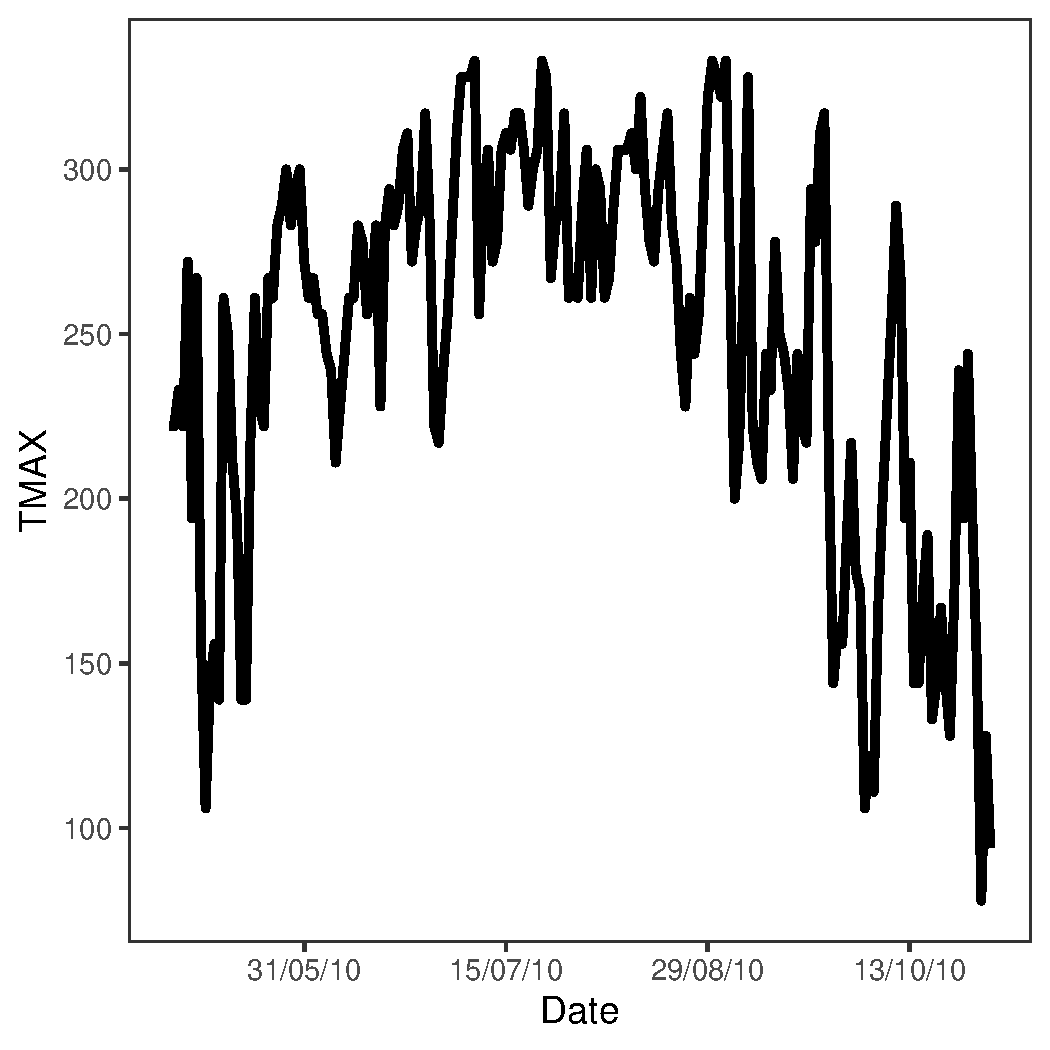
\includegraphics[width=\maxwidth]{figure/unnamed-chunk-8-1} 
\end{knitrout}
\subsection{Evaluating Records}

TBD

\subsection{Export Options}

TBD

\section{Sea Surface Temperature Data -- SURP PROJECT WAITING TO HAPPEN}

In contrast to terrestrial data, sea surface temperature (SST) is quite difficult to obtain and process. There are numerous tools to access the data, but they often require knowledge of complex software tools that are not easy to set up or programming experience with python or others.

\url{https://climexp.knmi.nl/select.cgi?id=someone@somewhere&field=ersstv5}

There are, however, a few tools build for R users that seem to accomplish all that we need. 

\url{https://rda.ucar.edu/index.html?hash=data_user&action=register}

\url{https://rda.ucar.edu/datasets/ds277.9/}

Alternatively, we can download flat ascII tables of gridded data:

\url{https://www1.ncdc.noaa.gov/pub/data/cmb/ersst/v5/ascii/}


\begin{knitrout}
\definecolor{shadecolor}{rgb}{0.969, 0.969, 0.969}\color{fgcolor}\begin{kframe}
\begin{alltt}
\hlkwd{library}\hlstd{(chron)}
\hlkwd{library}\hlstd{(RColorBrewer)}
\hlkwd{library}\hlstd{(lattice)}
\hlcom{#library(ncdf)}
\hlkwd{library}\hlstd{(ncdf4)}
\hlcom{#library(greenbrown) # for gridded trend analysis}

\hlstd{ersst.nc} \hlkwb{=} \hlstr{"/home/CAMPUS/mwl04747/github/Climate_Change_Narratives/Data/FA19/ersst.v5.185401.nc"}
\hlstd{Y1854} \hlkwb{=} \hlstr{"https://www1.ncdc.noaa.gov/pub/data/cmb/ersst/v5/ascii/ersst.v5.1854.asc"}
\hlstd{Y1864} \hlkwb{=} \hlstr{"https://www1.ncdc.noaa.gov/pub/data/cmb/ersst/v5/ascii/ersst.v5.1864.asc"}
\hlstd{Y1874} \hlkwb{=} \hlstr{"https://www1.ncdc.noaa.gov/pub/data/cmb/ersst/v5/ascii/ersst.v5.1874.asc"}
\hlstd{Y1884} \hlkwb{=} \hlstr{"https://www1.ncdc.noaa.gov/pub/data/cmb/ersst/v5/ascii/ersst.v5.1884.asc"}
\hlstd{Y1894} \hlkwb{=} \hlstr{"https://www1.ncdc.noaa.gov/pub/data/cmb/ersst/v5/ascii/ersst.v5.1894.asc"}
\hlstd{Y1904} \hlkwb{=} \hlstr{"https://www1.ncdc.noaa.gov/pub/data/cmb/ersst/v5/ascii/ersst.v5.1904.asc"}
\hlstd{Y1914} \hlkwb{=} \hlstr{"https://www1.ncdc.noaa.gov/pub/data/cmb/ersst/v5/ascii/ersst.v5.1914.asc"}
\hlstd{Y1924} \hlkwb{=} \hlstr{"https://www1.ncdc.noaa.gov/pub/data/cmb/ersst/v5/ascii/ersst.v5.1924.asc"}
\hlstd{Y1934} \hlkwb{=} \hlstr{"https://www1.ncdc.noaa.gov/pub/data/cmb/ersst/v5/ascii/ersst.v5.1934.asc"}
\hlstd{Y1944} \hlkwb{=} \hlstr{"https://www1.ncdc.noaa.gov/pub/data/cmb/ersst/v5/ascii/ersst.v5.1944.asc"}
\hlstd{Y1954} \hlkwb{=} \hlstr{"https://www1.ncdc.noaa.gov/pub/data/cmb/ersst/v5/ascii/ersst.v5.1954.asc"}
\hlstd{Y1964} \hlkwb{=} \hlstr{"https://www1.ncdc.noaa.gov/pub/data/cmb/ersst/v5/ascii/ersst.v5.1964.asc"}
\hlstd{Y1974} \hlkwb{=} \hlstr{"https://www1.ncdc.noaa.gov/pub/data/cmb/ersst/v5/ascii/ersst.v5.1974.asc"}
\hlstd{Y1984} \hlkwb{=} \hlstr{"https://www1.ncdc.noaa.gov/pub/data/cmb/ersst/v5/ascii/ersst.v5.1984.asc"}
\hlstd{Y1994} \hlkwb{=} \hlstr{"https://www1.ncdc.noaa.gov/pub/data/cmb/ersst/v5/ascii/ersst.v5.1994.asc"}
\hlstd{Y2004} \hlkwb{=} \hlstr{"https://www1.ncdc.noaa.gov/pub/data/cmb/ersst/v5/ascii/ersst.v5.2004.asc"}
\hlstd{Y2014} \hlkwb{=} \hlstr{"https://www1.ncdc.noaa.gov/pub/data/cmb/ersst/v5/ascii/ersst.v5.2014.asc"}

\hlstd{temp} \hlkwb{=} \hlkwd{rbind}\hlstd{(}\hlkwd{read.table}\hlstd{(Y1854)[}\hlnum{75}\hlstd{,}\hlnum{67}\hlstd{],} \hlkwd{read.table}\hlstd{(Y1864)[}\hlnum{75}\hlstd{,}\hlnum{67}\hlstd{],} \hlkwd{read.table}\hlstd{(Y1874)[}\hlnum{75}\hlstd{,}\hlnum{67}\hlstd{],}
\hlkwd{read.table}\hlstd{(Y1884)[}\hlnum{75}\hlstd{,}\hlnum{67}\hlstd{],} \hlkwd{read.table}\hlstd{(Y1894)[}\hlnum{75}\hlstd{,}\hlnum{67}\hlstd{],} \hlkwd{read.table}\hlstd{(Y1904)[}\hlnum{75}\hlstd{,}\hlnum{67}\hlstd{],}
\hlkwd{read.table}\hlstd{(Y1914)[}\hlnum{75}\hlstd{,}\hlnum{67}\hlstd{],} \hlkwd{read.table}\hlstd{(Y1924)[}\hlnum{75}\hlstd{,}\hlnum{67}\hlstd{],} \hlkwd{read.table}\hlstd{(Y1934)[}\hlnum{75}\hlstd{,}\hlnum{67}\hlstd{],}
\hlkwd{read.table}\hlstd{(Y1944)[}\hlnum{75}\hlstd{,}\hlnum{67}\hlstd{],} \hlkwd{read.table}\hlstd{(Y1954)[}\hlnum{75}\hlstd{,}\hlnum{67}\hlstd{],} \hlkwd{read.table}\hlstd{(Y1964)[}\hlnum{75}\hlstd{,}\hlnum{67}\hlstd{],}
\hlkwd{read.table}\hlstd{(Y1974)[}\hlnum{75}\hlstd{,}\hlnum{67}\hlstd{],} \hlkwd{read.table}\hlstd{(Y1984)[}\hlnum{75}\hlstd{,}\hlnum{67}\hlstd{],} \hlkwd{read.table}\hlstd{(Y1994)[}\hlnum{75}\hlstd{,}\hlnum{67}\hlstd{],}
\hlkwd{read.table}\hlstd{(Y2004)[}\hlnum{75}\hlstd{,}\hlnum{67}\hlstd{],} \hlkwd{read.table}\hlstd{(Y2014)[}\hlnum{75}\hlstd{,}\hlnum{67}\hlstd{])}

\hlstd{temp.df} \hlkwb{=} \hlkwd{data.frame}\hlstd{(}\hlkwc{Temp} \hlstd{=} \hlkwd{as.vector}\hlstd{(temp)}\hlopt{/}\hlnum{100}\hlstd{); temp.df}
\hlstd{temp.df}\hlopt{$}\hlstd{Year} \hlkwb{=} \hlkwd{seq}\hlstd{(}\hlnum{1854}\hlstd{,} \hlnum{2014}\hlstd{,} \hlnum{10}\hlstd{)}
\hlkwd{plot}\hlstd{(Temp}\hlopt{~} \hlstd{Year, temp.df)}
\hlkwd{abline}\hlstd{(}\hlkwd{coef}\hlstd{(}\hlkwd{lm}\hlstd{(Temp}\hlopt{~}\hlstd{Year,} \hlkwc{data}\hlstd{=temp.df)),} \hlkwc{col}\hlstd{=}\hlstr{"red"}\hlstd{)}
\hlcom{#automating this process!}

\hlstd{directory} \hlkwb{=} \hlstr{"/pub/data/cmb/ersst/v5/ascii"}

\hlstd{B195401} \hlkwb{=} \hlkwd{nc_open}\hlstd{(ersst.nc)}


\hlcom{# str(B195401)}
\hlcom{# print(B195401)}

\hlstd{ncin} \hlkwb{=} \hlstd{B195401}

\hlkwd{print}\hlstd{(ncin)}
\hlstd{lon} \hlkwb{<-} \hlkwd{ncvar_get}\hlstd{(ncin,} \hlstr{"lon"}\hlstd{)}
\hlstd{nlon} \hlkwb{<-} \hlkwd{dim}\hlstd{(lon)}
\hlkwd{head}\hlstd{(lon)}

\hlstd{lat} \hlkwb{<-} \hlkwd{ncvar_get}\hlstd{(ncin,} \hlstr{"lat"}\hlstd{,} \hlkwc{verbose} \hlstd{= F)}
\hlstd{nlat} \hlkwb{<-} \hlkwd{dim}\hlstd{(lat)}
\hlkwd{head}\hlstd{(lat)}

\hlkwd{print}\hlstd{(}\hlkwd{c}\hlstd{(nlon, nlat))}

\hlstd{t} \hlkwb{<-} \hlkwd{ncvar_get}\hlstd{(ncin,} \hlstr{"time"}\hlstd{)}
\hlstd{tunits} \hlkwb{<-} \hlkwd{ncatt_get}\hlstd{(ncin,} \hlstr{"time"}\hlstd{,} \hlstr{"units"}\hlstd{)}
\hlstd{nt} \hlkwb{<-} \hlkwd{dim}\hlstd{(t); nt}

\hlstd{lat.sel} \hlkwb{=} \hlnum{67}\hlstd{; lon.set} \hlkwb{=} \hlnum{75}

\hlcom{#ncvar_get(ncin, sst) #object 'sst' not found}

\hlcom{#ncvar_get(ncin, var$sst) object of type 'closure' is not subsettable}
\hlcom{#ncvar_get(ncin, var) second argument to ncvar_get must be an object of type ncvar or ncdim (both parts of the ncdf object returned by nc_open()), the character-string name of a variable or dimension or NA to get the default variable from the file.  If the file is netcdf version 4 format and uses groups, then the fully qualified var name must be given, for example, model1/run5/Temperature}

\hlkwd{ncvar_get}\hlstd{(ncin,} \hlstr{"sst"}\hlstd{)} \hlcom{#spits out the temperatures. but why the negative numbers!}

\hlcom{# tmp.array <- ncvar_get(ncin, dname) # doesn't work...}

\hlstd{tmp.array} \hlkwb{<-} \hlkwd{ncvar_get}\hlstd{(ncin,} \hlstr{"sst"}\hlstd{)}
\hlkwd{dim}\hlstd{(tmp.array)}

\hlstd{tmp.array[}\hlnum{75}\hlstd{,} \hlnum{67}\hlstd{]}

\hlstd{tmp.array[}\hlnum{67}\hlstd{,]}

\hlstd{dlname} \hlkwb{<-} \hlkwd{ncatt_get}\hlstd{(ncin,} \hlstr{"sst"}\hlstd{,} \hlstr{"long_name"}\hlstd{)}
\hlstd{dunits} \hlkwb{<-} \hlkwd{ncatt_get}\hlstd{(ncin,} \hlstr{"sst"}\hlstd{,} \hlstr{"units"}\hlstd{)}
\hlstd{fillvalue} \hlkwb{<-} \hlkwd{ncatt_get}\hlstd{(ncin,} \hlstr{"sst"}\hlstd{,} \hlstr{"_FillValue"}\hlstd{)}
\hlkwd{dim}\hlstd{(tmp.array)}

\hlstd{title} \hlkwb{<-} \hlkwd{ncatt_get}\hlstd{(ncin,} \hlnum{0}\hlstd{,} \hlstr{"title"}\hlstd{)}
\hlstd{institution} \hlkwb{<-} \hlkwd{ncatt_get}\hlstd{(ncin,} \hlnum{0}\hlstd{,} \hlstr{"institution"}\hlstd{)}
\hlstd{datasource} \hlkwb{<-} \hlkwd{ncatt_get}\hlstd{(ncin,} \hlnum{0}\hlstd{,} \hlstr{"source"}\hlstd{)}
\hlstd{references} \hlkwb{<-} \hlkwd{ncatt_get}\hlstd{(ncin,} \hlnum{0}\hlstd{,} \hlstr{"references"}\hlstd{)}
\hlstd{history} \hlkwb{<-} \hlkwd{ncatt_get}\hlstd{(ncin,} \hlnum{0}\hlstd{,} \hlstr{"history"}\hlstd{)}
\hlstd{Conventions} \hlkwb{<-} \hlkwd{ncatt_get}\hlstd{(ncin,} \hlnum{0}\hlstd{,} \hlstr{"Conventions"}\hlstd{)}

\hlcom{# split the time units string into fields}
\hlstd{tustr} \hlkwb{<-} \hlkwd{strsplit}\hlstd{(tunits}\hlopt{$}\hlstd{value,} \hlstr{" "}\hlstd{)}
\hlstd{tdstr} \hlkwb{<-} \hlkwd{strsplit}\hlstd{(}\hlkwd{unlist}\hlstd{(tustr)[}\hlnum{3}\hlstd{],} \hlstr{"-"}\hlstd{)}
\hlstd{tmonth} \hlkwb{=} \hlkwd{as.integer}\hlstd{(}\hlkwd{unlist}\hlstd{(tdstr)[}\hlnum{2}\hlstd{])}
\hlstd{tday} \hlkwb{=} \hlkwd{as.integer}\hlstd{(}\hlkwd{unlist}\hlstd{(tdstr)[}\hlnum{3}\hlstd{])}
\hlstd{tyear} \hlkwb{=} \hlkwd{as.integer}\hlstd{(}\hlkwd{unlist}\hlstd{(tdstr)[}\hlnum{1}\hlstd{])}
\hlkwd{chron}\hlstd{(t,} \hlkwc{origin} \hlstd{=} \hlkwd{c}\hlstd{(tmonth, tday, tyear))}

\hlcom{# tmp.array[tmp.array == fillvalue$value] <- NA}

\hlcom{# length(na.omit(as.vector(tmp.array[, , 1])))}

\hlstd{m} \hlkwb{<-} \hlnum{1}
\hlstd{tmp.slice} \hlkwb{<-} \hlstd{tmp.array[, , m]}

\hlkwd{image}\hlstd{(lon, lat, tmp.array,} \hlkwc{col} \hlstd{=} \hlkwd{rev}\hlstd{(}\hlkwd{brewer.pal}\hlstd{(}\hlnum{10}\hlstd{,} \hlstr{"RdBu"}\hlstd{)))}

\hlcom{# image(lon, lat, tmp.slice, col = rev(brewer.pal(10, "RdBu")))}
\end{alltt}
\end{kframe}
\end{knitrout}

\section{Satellite Data}

TBD

\section{Ice-Core Data}

TBD



\end{document}
